\documentclass{tufte-handout}

\usepackage{../CommonLatexPackages/fall2018_preamble_v1.0}
\fancypagestyle{firstpage}


\title{The Gauntlet}

\author{Quantitative Engineering Analysis}
\date{Spring 2019}


\begin{document}

\maketitle
\thispagestyle{firstpage}

\section{Overview}
You have mastered the Bridge of Doom\texttrademark~and navigated Flatland\texttrademark.  Now you face the most challenging challenge you've ever been challenged with.  In this final challenge, you will help your robot to dodge through obstacles on your way to the ultimate prize -- knowledge.

Throughout this semester, you have applied many quantitative engineering analysis tools. For this challenge, you'll use a powerful new sensor (the laser scanner), explore some new algorithms for optimization, and use the mathematics of artificial potential functions.

You will work with a partner to complete the challenge \emph{and} the write-up.

\subsection{Learning Goals}
\begin{marginfigure}
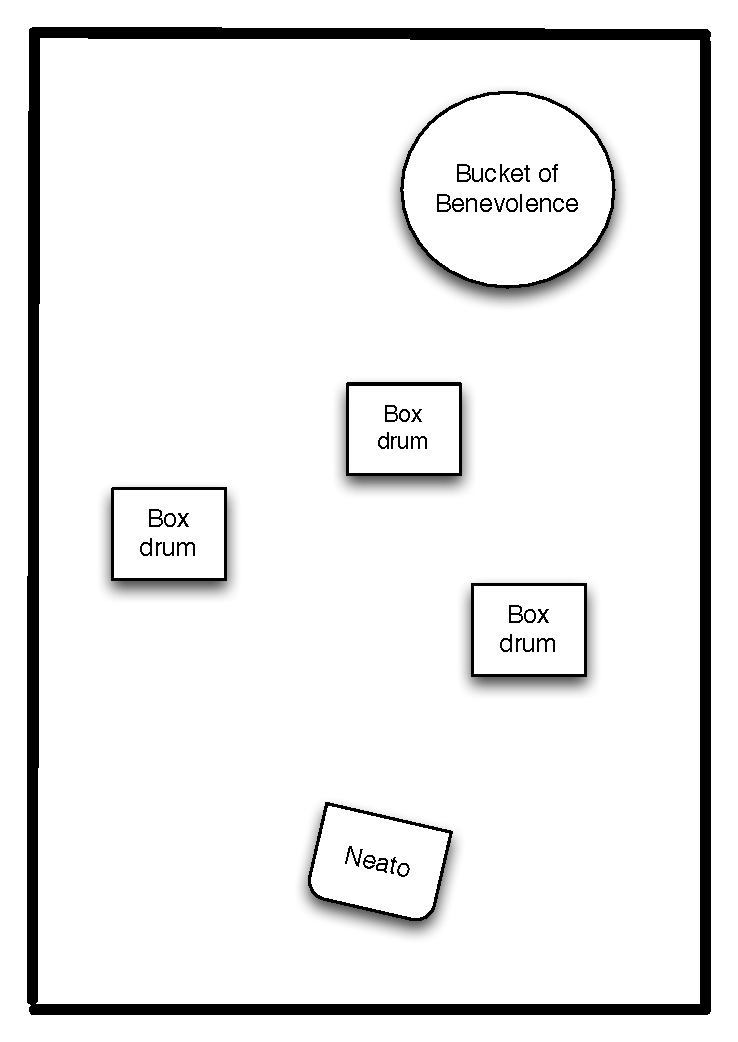
\includegraphics[width=\linewidth]{Figures/gauntlet}
\caption{A top-down view of The Gauntlet\texttrademark.  You should write a program to guide the Neato past the obstacles (the box drums) to the goal (the Bucket of Benevolence\texttrademark).\label{fig:gauntlet}}
\end{marginfigure}
By the end of this challenge, you should be comfortable with the following:
\begin{enumerate}
\item Fitting geometrical models to laser scan data.
\item Outlier resistant techniques for optimization.
\item Potential functions and vector fields.
\item Basic obstacle avoidance and path planning.
\item Working with multiple coordinate systems.
\end{enumerate}

\section{The Challenge}

Your goal is to write a program to pilot your robot through a series of obstacles (walls and box drums).  You will detect these obstacles using your robot's onboard laser scanner, which can detect obstacles within a 3m range (see Figure~\ref{fig:gauntlet}).

This final QEA-I challenge has a hierarchy of missions, which get progressively more difficult. For all missions, the goal is to gently tap the Bucket of Benevolence (BoB). Here are the conditions for the missions:
\begin{enumerate}
%\item You are given the coordinates of the BoB. The only obstacles are the walls.
\item [Level 1] You are given the coordinates of the BoB. You are given a map of the obstacle locations (walls and box drums). The path can be entirely pre-planned.
\item [Level 2] You are given the coordinates of the BoB, but you must use the LIDAR to detect and avoid obstacles. 
\item [Level 3] You are given the radius of the BoB, but not the coordinates. You must use the LIDAR to detect and avoid obstacles and identify and locate the BoB. To identify the BoB, you will need to differentiate the distinctive, circular shape of the goal from the linear shape of the obstacles  (see Figure~\ref{fig:gauntlet}). If you choose this mission, we recommend you look at the circle-fitting extension at the end of Day 7 for guidance.
\end{enumerate}

To achieve whichever mission(s) you choose to accept, you will apply what you have learned about potential functions and vector fields.  You may also choose to extend any of the above missions by applying or creating another goal-seeking/obstacle-avoiding algorithm, not taking the BoB's radius as an input, or trying to reach the target as soon as quickly as possible.

\section{Deliverables}

\newthought{DUE next class (Thursday 5/2, 9 AM) [6 pts]:}

To ensure you make significant progress on the math side of this project before the last class on Thursday, we ask you to turn in (as a pair!) a document with the following plots:
\be
\item A map of the pen, collected by LIDAR, with walls and obstacles fitted as line segments using your RANSAC algorithm. A fit for the BoB is optional. [2 pts]
\item An equation and a contour (or 3-D) plot of the potential field you developed for the pen. [2 pts]
\item A quiver plot of the gradient of your potential field. [1 pt]
\item A path of gradient descent from the starting point to the BoB. [1 pt]
\ee

These plots should be clearly labeled so we know exactly what we're looking at.


\newthought{DUE at the final event (Tuesday 5/7, 8 AM) [8 pts]:}

\emph{Together with your partner,} prepare a video and a {\bf brief} writeup of your work on this challenge. That's right, you and your partner only need to turn in one report! Wow. The Bucket of Benevolence runneth over. 

Your final writeup should center around critical information and informative figures. It can be as short as you want, but it must contain the following components:
\begin{enumerate}
%\item Your answers to all of the exercises in this document.
\item A short introduction stating the mission you chose and a brief summary of the strategy you used to solve the challenge. You might find it helpful to refer to the decomposition exercise from Day 7. [1 pt]
\item Some experimental data that shows, quantitatively, how well your system worked, plus a few sentences of explanation. 
\be
\item The time it took your robot to get to the BoB (for whichever mission you choose) and the distance it traveled. [1 pt]
\item A plot with: a LIDAR scan of the pen,  the intended path of gradient descent, and the path your robot took (calculated from the wheel encoder data). This should be a legible plot with axis labels, a legend, and a caption...the works. [3 pts]
\ee
\item A link to a video of your robot in action. It should, at the minimum, clearly show your robot performing the chosen challenge, but we encourage you to create a fun video to share with the class on the final event day! [2 pts]
\end{enumerate}

In addition to the writeup, you should also turn in your (commented and readable!) code. [1 pt]


\end{document} 
